\documentclass[a4paper, 14pt,russian]{extarticle}

\usepackage[russian]{babel}
\usepackage[T2A]{fontenc}
\usepackage[utf8]{inputenc}
%Соответствующий математический шрифт для Times new roman
\usepackage{newtxmath}
\usepackage{fontspec} 
\usepackage{multirow}
%\usepackage{polyglossia}
%Times new roman
\defaultfontfeatures{Ligatures={TeX},Renderer=Basic} 
\setmainfont[Ligatures={TeX,Historic}]{Times New Roman}
\setmainfont{Times New Roman}
\setsansfont{Arial}
\setmonofont{Courier New}
\newfontfamily\cyrillicfont[Script=Cyrillic]{Times New Roman}
\newfontfamily\cyrillicfontsf[Script=Cyrillic]{Arial}
\newfontfamily\cyrillicfonttt[Script=Cyrillic]{Courier New}

%\setdefaultlanguage{russian}

%Геометрия
\usepackage{geometry}
\geometry{top=20mm}
\geometry{bottom=15mm}
\geometry{left=20mm}
\geometry{right=15mm}
\usepackage{setspace}
%Нормальные дроби через запятую
\usepackage{ncccomma}

\newcommand{\changefont}{%
	\fontsize{12}{11}\selectfont
}

%Заголовки
\usepackage{fancyhdr}
\pagestyle{fancy}
\fancyhf{}
%\renewcommand{\sectionmark}[1]{\markright{#1}}
\fancyhead[R]{\changefont \slshape \leftmark}
\fancyhead[L]{\changefont \slshape \rightmark}
%\newcommand{\ssubsection}[1]{\subsection*{#1}
%	\addcontentsline{toc}{subsection}{#1}
%	\markright{#1}{}}
\cfoot{\thepage}

%\полуторный интервал
\setstretch{1.15}
\setlength{\parindent}{1.25cm}

\usepackage{amsmath, amsfonts, mathtools}
\usepackage{physics}
\usepackage{indentfirst}
\usepackage{xcolor}
\usepackage{alltt}
\usepackage{graphicx}
\usepackage{wrapfig}
\usepackage{pgfplots}
\usepackage{filecontents}

%Настройка ссылок
\usepackage{hyperref}
%\usepackage{upgreek}
%\renewcommand{\beta}{\upbeta}
\hypersetup{
	colorlinks,
	citecolor=black,
	filecolor=black,
	linkcolor=black,
	urlcolor=black
}
\usepackage{caption}
\DeclareCaptionLabelSeparator{dot}{. }
\captionsetup{justification=centering,labelsep=dot}
\usepackage{titlesec}

%Формат заголовков
\titleformat{\section}{\bfseries\filcenter\Large}{\thesection}{1em}{}
\titleformat{\subsection}{\bfseries\filcenter\large}{\thesubsection}{1em}{}
\titleformat{\subsubsection}{\bfseries\filcenter\normalsize}{\thesubsubsection}{1em}{}

\usepackage{chngcntr}

%Включить в нумерацию картинок раздел
\counterwithin{figure}{section}

%Листинги кода и их стили
\usepackage{listings}
%\usepackage{minted}
\lstdefinestyle{c++} {
	language=C++,
	breaklines=true,
	frame=single,
	numbers=left,
	basicstyle=\footnotesize\ttfamily,
	keywordstyle=\bfseries\color{green!40!black},
	commentstyle=\itshape\color{purple!40!black},
	identifierstyle=\color{blue},
	backgroundcolor=\color{gray!10!white},
}

\lstdefinestyle{python}{
	language=Python,
	breaklines=true,
	frame=single,
	numbers=left,
	keywordstyle=\bfseries\color{green!40!black},
	frame=lines,
	basicstyle=\footnotesize\rmfamily
}

\lstdefinestyle{cmd}{
	breaklines=true,
	frame=single,
	basicstyle=\footnotesize\ttfamily,
	frame=lines
	basicstyle=\footnotesize
}
\usepackage{tikz}
\usepackage{tkz-base}
\usetikzlibrary{quotes,angles}
\usetikzlibrary {arrows.meta}
%\usepackage{tkz-euclide}
\usetikzlibrary{calc}
\usetikzlibrary{shapes.geometric, shapes.misc, arrows}

\tikzstyle{startstop} = [rectangle, rounded corners, 
minimum width=3cm, 
minimum height=1cm,
text centered, 
draw=black]

\tikzstyle{io} = [trapezium, 
trapezium stretches=true, % A later addition
trapezium left angle=70, 
trapezium right angle=110, 
minimum width=3cm, 
minimum height=1cm, text centered, 
draw=black]

\tikzstyle{process} = [rectangle, 
minimum width=3cm, 
minimum height=1cm, 
text centered, 
text width=5cm, 
draw=black]

\tikzstyle{decision} = [diamond, 
minimum width=3cm, 
minimum height=1cm, 
text centered, 
draw=black]

\tikzstyle{startfor} = [chamfered rectangle, 
chamfered rectangle corners={north west, north east},
minimum width=3cm, 
minimum height=1cm, 
text centered, 
draw=black]

\tikzstyle{endfor} = [chamfered rectangle, 
chamfered rectangle corners={south west, south east},
minimum width=3cm, 
minimum height=1cm, 
text centered, 
draw=black]

\tikzstyle{block} = [style=draw, 
	minimum width = 1.6cm,
	minimum height = 1.2cm]
\tikzstyle{arrow} =[-{Latex[length=3mm]}, thick]

\newcommand{\drawsum}[2]{\node[draw,
	circle,
	minimum size=1cm
	] (#1) at #2{};
	\draw (#1.north east) -- (#1.south west)
	(#1.north west) -- (#1.south east)}

\newcommand{\fillsumsouth}[1]{\draw[fill=black] (#1.center) -- ++(-135:0.5cm) arc (-135:-45:0.5cm) -- cycle}
\newcommand{\fillsumnorth}[1]{\draw[fill=black] (#1.center) -- ++(135:0.5cm) arc (135:45:0.5cm) -- cycle}

\begin{document}
	
	\begin{titlepage}
	\newpage
	\begin{center}
		
\includegraphics[width=\textwidth]{png/tit.png}
		Институт информационных и вычислительных технологий \\
			Кафедра управления и интеллектуальных технологий
		\vspace{1.25cm}
	\end{center}
	
	\vspace{1.2em}
	
	\begin{center}
		%\textsc{\textbf{}}
		\begin{spacing}{1}
			{\Large Отчёт по лабораторной работе №2 \linebreak
			По дисциплине <<Моделирование систем управления>> \\}
			\large{\bf<<Моделирование многосвязных систем и исследование
				устойчивости линейных систем>>}
		\end{spacing}
	\end{center}
	
	\vspace{5em}
	

	\vspace{6em}
	
		\noindent Выполнили студенты: Михайловский М., Рехалов А. \\
		Группа: А-03-21 \\
		Бригада: 1\\
		Проверил: Васильев А.\,А.
	
	
	\vspace{\fill}
	
	\begin{center}
		Москва 2024
	\end{center}
	
\end{titlepage}
	\pagenumbering{arabic}
	\setcounter{page}{2}
	\tableofcontents
	\newpage
	
	\newcommand{\diag}[1]{\mathrm{diag}\,#1}
	\renewcommand{\sp}[1]{\mathrm{sp}\,#1}
	\newcommand{\res}[1]{\underset{#1}{\mathrm{res}}}

	\section{Подготовка к работе}
	\subsection{Основные положения}
	
	Пусть имеется нелинейная модель системы, представленная в виде (\ref{sys}). 
	\begin{equation}
		\begin{cases}
			\dot{x} = \varphi(x),\;\text{где }x\in\mathbb{R}^n \\
			x(0) = x_0	
		\end{cases}
		,\;\varphi: \mathbb{R}^n \mapsto \mathbb{R}^n
		\label{sys}
	\end{equation}
	
	Рассматривается задача понижения размерности такой модели при некоторых вводимых ограничениях. В данном случае будем рассматривать понижение размерности данной модели на некотором временном подынтервале $[T_\text{гр},\,T_\text{кон}]\subset [0, T_\text{кон}]$.
	
	Рассмотрим линеаризованную модель:
	\begin{equation*}
		\dot{x}(t) \approx x(T_i) + J_\varphi (T_i)\cdot (x(t) - x(T_i)),\;\text{где }J_\varphi (T_i)\text{ -- матрица Якоби функции \varphi(x)}
	\end{equation*}
	
	Применим оператор конечной разности $\Delta$:
	\begin{equation}
		\dot{\Delta x} \approx J\varphi (T_i)\cdot \Delta x
		\label{lin}
	\end{equation}
	
	Получили линеаризованную модель в отклонениях. Исходя из параметров матрицы Якоби в точке $x(T_i)$, можно определить является ли исходная модель в области $x\in X_i$ близкой к $x(T_i)$ сингулярно-возмущённой. 
	
	Условием принадлежности рассматриваемой модели этому классу будет наличие такого собственного числа $p^{(i)}\in \sp{J_\varphi (T_i)}: \mathrm{Re}\,p^{(i)}\to -\infty$. На практике рассматривается наличие собственных значений $p^{(i)}$ сильно удалённых от остальных:
	\begin{equation}
		\frac{\left| \mathrm{Re}\,p^{(i)} \right|}{\;\left| \min\limits_{p_0 \in \sp{J_\varphi (T_i)}\setminus \Lambda} \mathrm{Re}\,p_0 \right|\;}\geq 10
		\label{sing_usl}
	\end{equation} 
	
	Где $\Lambda$ -- наиболее выделяющиеся собственные значения.
	
	Для функции вида $\varphi(x) = Cx + f(x)$, где $i$-ая функция $f_i (x)$ линейна по $x_i$, то есть $\pdv{f_i}{x_i} \equiv 0$ условие (\ref{sing_usl}) -- это необходимое и достаточное условие принадлежности (\ref{sys}) к классу сингулярно-возмущённых в области $x\in X_i$.
	
	Для $\varphi(x)$ общего вида эти условия носят лишь необходимый характер.
	
	\subsection{Линеаризация системы}
	
	Дана система следующего вида:
	\begin{equation}
		\begin{cases}
			\dot{x}_1 = a_{11} x_1 + a_{12} x_2 + a_{13} x_3 + b_1 (1+s) y_1 \\
			\dot{x}_2 a_{21} x_1 + a_{22} x_2 + a_{23} x_3 + b_2 u_1 \\ 
			\dot{x}_3 = a_{31} x_1 + a_{32} x_2 + a_{33} x_3 \\
			\dot{y}_1 = a_{44} y_1 + a_{45} y_2 + b_3 (1+s) x_1 \\
			\dot{y}_2 = a_{54} y_1 + a_{55} y_2 \\
			\dot{z}_1 = a_{67} z_2 \\
			\dot{z}_2 = a_{78} z_3 \\
			\dot{z}_3 = a_{86} z_1 + a_{87} z_2 + a_{88} z_3 + c_1 M_0 + b_4 s \\
			\dot{u}_1 = a_{9,\,10} u_2 + c_2 U_0 \\
			\dot{u}_2 = a_{10,\,11} u_3 + c_3 U_0 \\
			\begin{multlined}
				\dot{u}_3 = a_{11,\,9} u_1 + a_{11,\,10} u_2 + a_{11,\,11} u_3 + c_4 U_0 + b_5 + \\[-3ex] + \sqrt{ (d_1 x_1 + d_2 x_2 + d_3 x_3)^2 + (d_4 y_1 + d_5 y_2)^2 }	
			\end{multlined}
			 \\
			\dot{s} = a_{12,\,6} z_1 + a_{12,\,1} x_1(e_1 y_1 + e_2 y_2) + a_{12,\,4} y_1 (e_3 x_1 + e_4 x_2 + e_5 x_3)
		\end{cases}
		\label{sys_eq}
	\end{equation}
	
	Рассчитаем матрицу Якоби от вектор-функции $\varphi(x)$ задающей правую часть системы при нулевых входных воздействиях $M_0$ и $U_0$:
	\setcounter{MaxMatrixCols}{20}
	\begin{equation}
		\scalemath{0.9}{
		J_\varphi = \begin{bmatrix}
			a_{11} & a_{12} & a_{13} & b_1(1+s) & 0 & 0 & 0 & 0 & 0 & 0 & 0 & b_1 y_1 \\
			a_{21} & a_{22} & a_{23} & 0 & 0 & 0 & 0 & 0 & b_2 & 0 & 0 & 0 \\
			a_{31} & a_{32} & a_{33} & 0 & 0 & 0 & 0 & 0 & 0 & 0 & 0 & 0 \\
			b_3(1 + s) & 0 & 0 & a_{44} & a_{45} & 0 & 0 & 0 & 0 & 0 & 0 & b_3 x_1 \\
			0 & 0 & 0 & a_{54} & a_{55} & 0 & 0 & 0 & 0 & 0 & 0 & 0 \\
			0 & 0 & 0 & 0 & 0 & 0 & a_{67} & 0 & 0 & 0 & 0 & 0 \\
			0 & 0 & 0 & 0 & 0 & 0 & 0 & a_{78} & 0 & 0 & 0 & 0 \\
			0 & 0 & 0 & 0 & 0 & a_{86} & a_{87} & a_{88} & 0 & 0 & 0 & b_4 \\
			0 & 0 & 0 & 0 & 0 & 0 & 0 & 0 & 0 & a_{9,\,10} & 0 & 0 \\
			0 & 0 & 0 & 0 & 0 & 0 & 0 & 0 & 0 & 0 & a_{10,\,11} & 0 \\
			g_1 & g_2 & g_3 & g_4 & g_5 & 0 & 0 & 0 & a_{11,\,9} & a_{11,\,10} & a_{11,\,11} & 0 \\
			h_1 & h_2 & h_3 & h_4 & h_5 & a_{12,\,6} & 0 & 0 & 0 & 0 & 0 & 0 
		\end{bmatrix} }
		\label{jacobi}
	\end{equation}
	
	Где $g_1,\; g_2,\; g_3,\; g_4,\; g_5,\; h_1,\; h_2,\; h_3,\; h_4,\; h_5$:
	\begin{equation*}
		g_1 = \frac{b_5 d_1 r_x}{m},\; g_2 = \frac{b_5 d_2 r_x}{m},\; g_3 = \frac{b_5 d_3 r_x}{m},\; g_4 = \frac{b_5 d_4 r_x}{m},\; g_5 = \frac{b_5 d_5 r_x}{m} 
	\end{equation*}
	\begin{equation*}
		r_x = \sqrt{ (d_1 x_1 + d_2 x_2 + d_3 x_3)^2 + (d_4 y_1 + d_5 y_2)^2 }
	\end{equation*}
	\begin{equation*}
		h_1 = a_{12,\,1} (e_1 y_1 + e_2 y_2) + a_{12,\,4} e_3 y_1,\; h_2 = a_{12,\,4} e_4 y_1,\; h_3 = a_{12,\,4} e_5 y_1
	\end{equation*}
	\begin{equation*}
		h_4 = a_{12,\,1} e_1 x_1 + a_{12,\,4} (e_3 x_1 + e_4 x_2 + e_5 x_3),\; h_5 = a_{12,\,1} e_2 x_1
	\end{equation*}

	\section{Выполнение работы}
	\vspace{-3ex}
	\subsection{Моделирование системы}
	
	В рассматриваемой системе (\ref{sys_eq}) параметры имеют следующие значения:
	\begin{align*}
		&a_{11} = -2071,132,\;a_{12} = 1014,733,\; a_{13} = 1014,733,\; b_1 = 314, \\
		&a_{21} = 3,034,\; a_{22} = -6,193,\; a_{23} = 3,34,\; b_2 = 0,378, \\
		&a_{31} = 78,069,\; a_{32} = 78,069,\; a_{33} = -159,344, \\
		&b_3 = -314,\; a_{44} = -1606,256,\; a_{45} = 1479,609, \\
		&a_{54} = 97,310,\; a_{55} = -105,64, \\
		&a_{67} = 1,\; a_{78} = 1,\; a_{86} = -33949,6,\; a_{87} = -6989,92,\; a_{88} = -45, \\
		&c_1 = 2000,\; b_4 = -100000,\; a_{9,\,10} = 1,\; c_2 = 33,33, \\
		&a_{10,\,11} = 1,\; c_3 = 2777,777,\; a_{11,\,9} = -55555,55, \\
		&a_{11,\,10} = -4444,44,\; a_{11,\,11} = -116,66,\; c_4 = 16666,66, \\
		&b_5 = -444444,44,\; d_1 = 8,18,\; d_2 = -4,01,\; d_3 = -4,01,\; d_3 = 6,347,\; d_5 = -5,847, \\
		&a_{12,\,6} = 0,303,\; a_{12,\,1} = -1,77,\; a_{12,\,4} = 1,215, \\
		&e_1 = 1,0856,\; e_2 = -1,\; e_3 = 2,041,\; e_4 = -1,\; e_5 = -1
	\end{align*}
	
	Для моделирования такой системы соберём схему, представленную на рис. \ref{scheme1}. Код, заданный в программируемом блоке, приведён в листинге \ref{listing1}.
	
	\begin{figure}[!h]
		\centering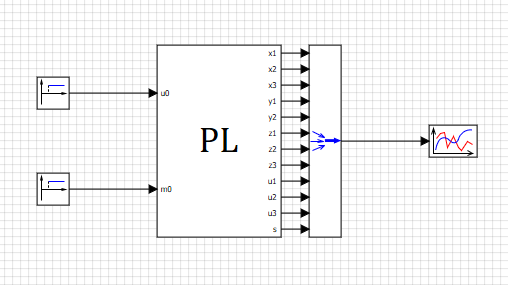
\includegraphics[width=.65\textwidth]{png/scheme1.png}
		\caption{Схема для моделирование переходных процессов в системе (\ref{sys_eq})}
		\label{scheme1}
	\end{figure}
	
	\begin{listing}
		\captionof{lstlisting}{Код для моделирования системы (\ref{sys_eq})}
		\label{listing1}
		\begin{minted}[
		frame=lines,fontsize=\footnotesize,breaklines=true,numbers=left
		]{Modelica}
input U0, M0;

init x1 = 0, x2 = 0, x3 = 0, y1 = 0, y2 = 0, z1 = 0, z2 = 0, z3 = 0, u1 = 0, u2 = 0, u3 = 0, s = 0;

output x1, x2, x3, y1, y2, z1, z2, z3, u1, u2, u3, s;

x1' = -2071.132*x1 + 1014.733*x2 + 1014.733 * x3 + (314 + 314*s)*y1;
x2' = 3.034*x1 - 6.193*x2 + 3.34*x3 + 0.378*u1;
x3' = 78.069*x1 + 78.069*x2 - 159.344*x3;
y1' = -1606.256*y1 + 1479.609*y2 + (-314 - 314*s)*x1;
y2' = 97.310*y1 - 105.640*y2;
z1' = z2;
z2' = z3;
z3' = -33949.6*z1 - 6989.92*z2 - 45*z3 + 2000*M0 - 100000*s;
u1' = u2 + 33.33*U0;
u2' = u3 + 2777.777*U0;
u3' = -55555.55*u1 - 4444.44*u2 - 116.66*u3 + 16666.66*U0 - 44444.44*sqrt( (8.18000000*x1 - 4.0100000*x2 - 4.010000*x3) * (8.18000000*x1 - 4.0100000*x2 - 4.010000*x3) + (6.34700000*y1 - 5.847000*y2) * (6.34700000*y1 - 5.847000*y2) );
s'  = 0.303*z1 - 1.77*x1*(1.0856*y1 - y2) + 1.215*y1*(2.041*x1 - x2 - x3);
		\end{minted}
	\end{listing}
		
	\begin{figure}[!h]
		\begin{subfigure}{.5\textwidth}
			\centering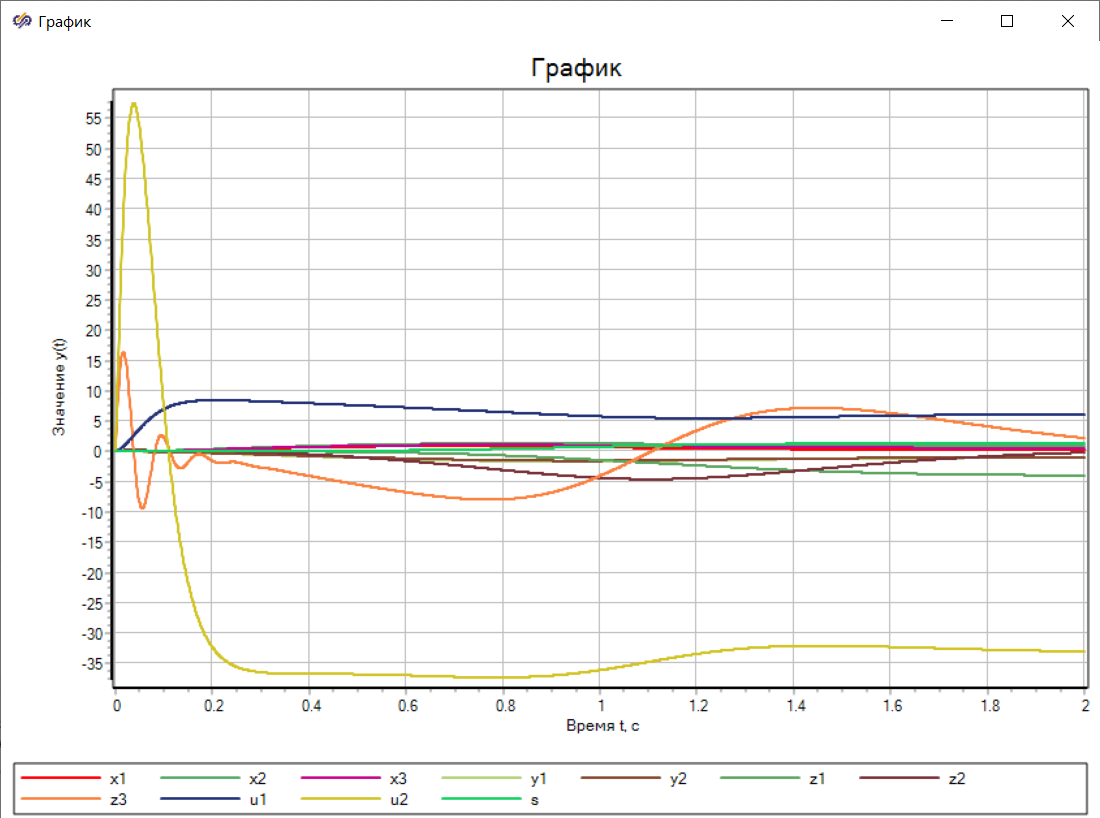
\includegraphics[width=.95\textwidth]{png/graph1.1.png}
			\caption{}
		\end{subfigure}
		\begin{subfigure}{.5\textwidth}
			\centering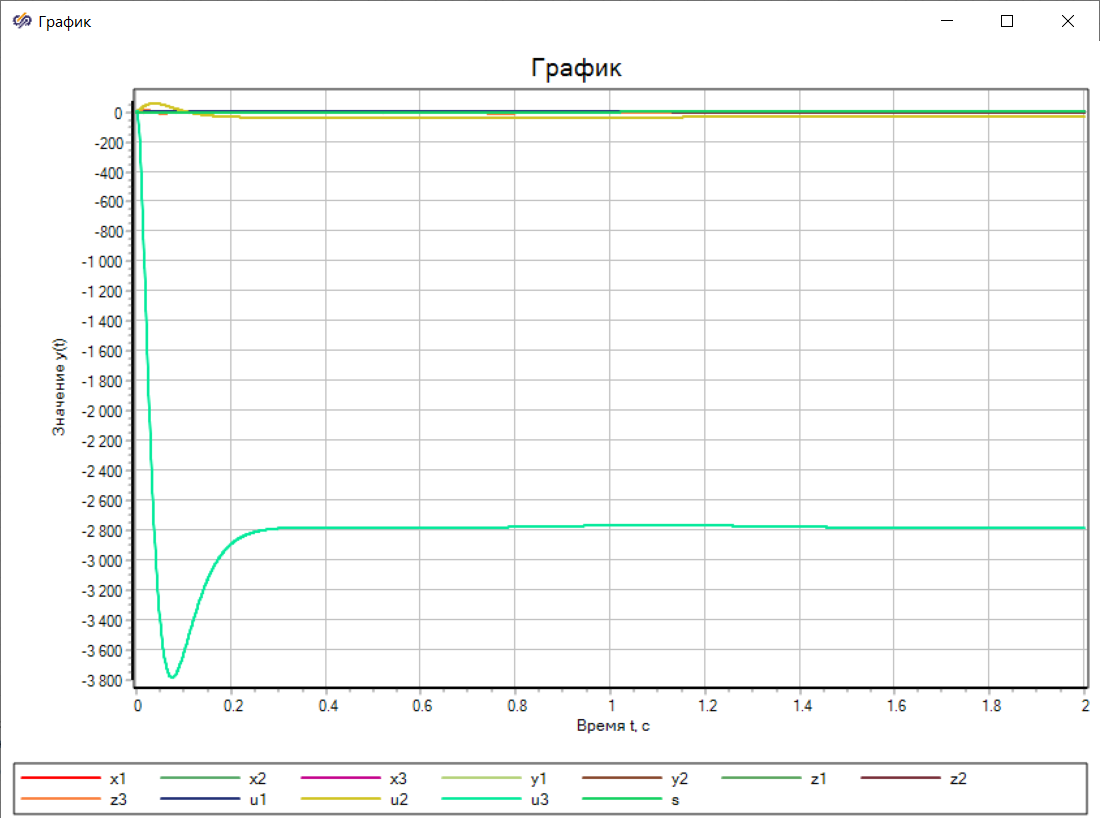
\includegraphics[width=.95\textwidth]{png/graph1.2.png}
			\caption{}
		\end{subfigure}
		\caption{Переходные процессы в системе: а) скрыта переменная $u_3$ б) показана переменная $u_3$}
		\label{graph1} 
	\end{figure}
	
	В результате моделирования при нулевых начальных условиях, получили переходные процессы, представленные на рис. \ref{graph1}. Как видим, переменные состояния изменяются с разным характером и имеют разный порядок. Также стоит отметить, что исследуемая система устойчива по входному ступенчатому воздействию.
	
	Теперь смоделируем свободное движение из установившегося режима предыдущего моделирования. Для этого изменим схему: рис. \ref{scheme2}.
	
	\begin{figure}[h]
		\centering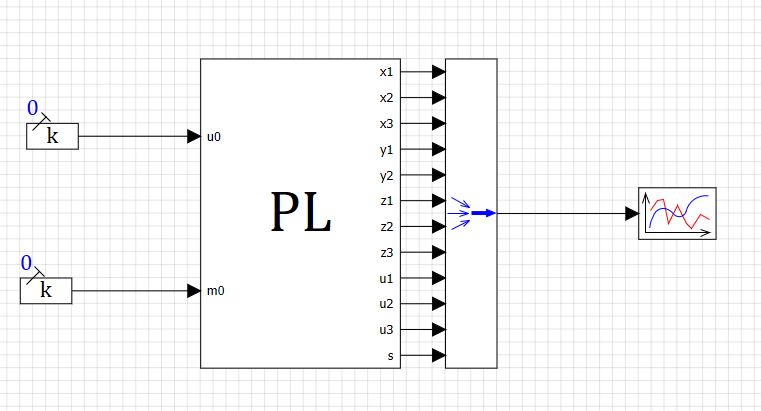
\includegraphics[width=.65\textwidth]{png/scheme2.png}
		\caption{Схема для моделирования свободного движения}
		\label{scheme2}
	\end{figure}
	
	В программируемом блоке изменим начальные условия в соответствии со значениями, полученными в результате предыдущего моделирования. Для этого изменим строку 3 на:
	\begin{listing}[h]
		\begin{minted}[
			frame=lines,fontsize=\footnotesize,breaklines=true
			]{Modelica}
init x1 = 0.3693614, x2 = 0.89470902, x3 = 0.61931999, y1 = -1.0820844, y2 = -0.99675911, z1 = -3.682321, z2 = -4.615e-8, z3 = 1.16e-7, u1 = 6.2215701, u2 = -33.33, u3 = -2777.777, s = 1.2701333;
		\end{minted}
	\end{listing}
	
	\begin{figure}[!h]
		\begin{subfigure}{.5\textwidth}
			\centering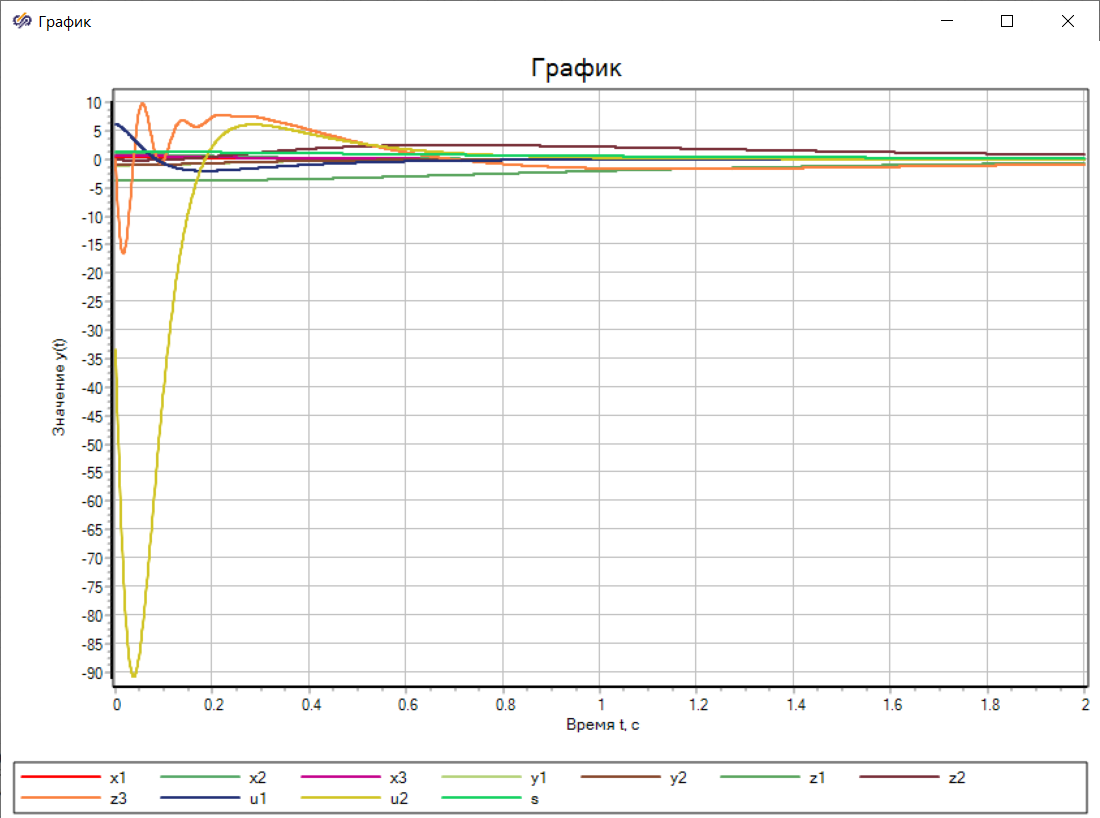
\includegraphics[width=.95\textwidth]{png/graph2.1.png}
			\caption{}
		\end{subfigure}
		\begin{subfigure}{.5\textwidth}
			\centering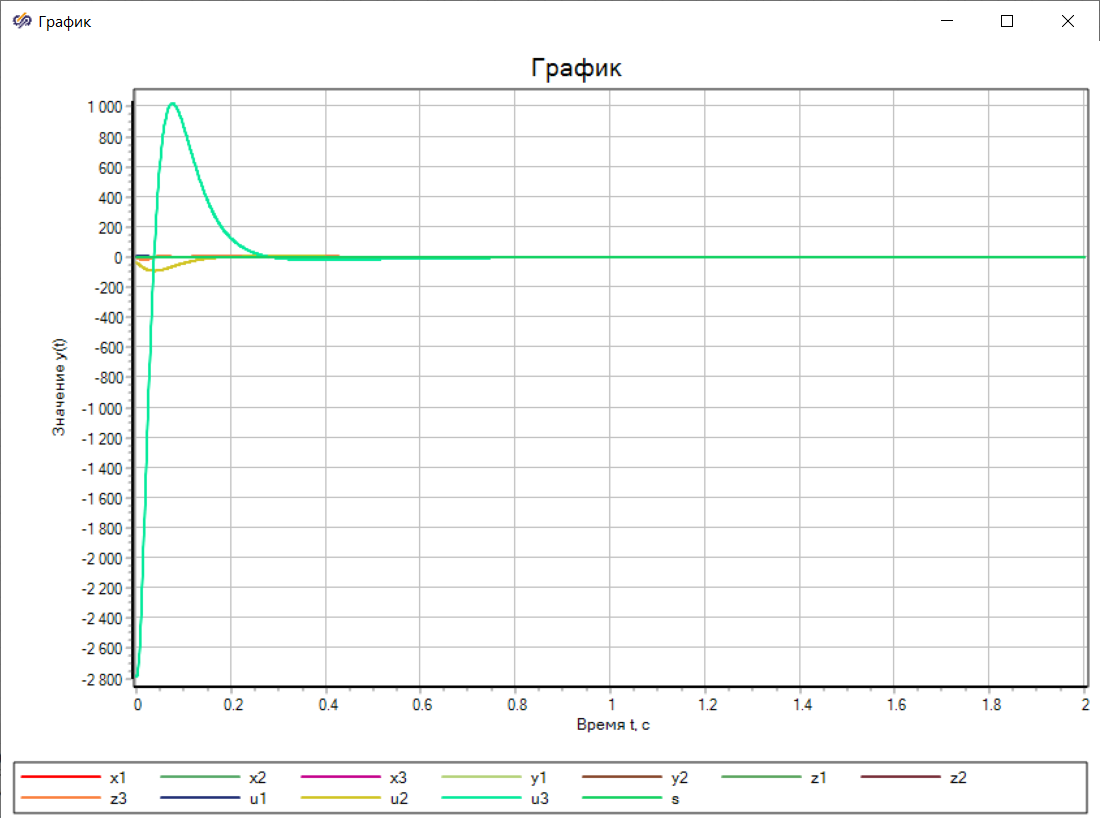
\includegraphics[width=.95\textwidth]{png/graph2.2.png}
			\caption{}
		\end{subfigure}
		\caption{Свободное движение в системе: а) скрыта переменная $u_3$ б) показана переменная $u_3$}
		\label{graph2} 
	\end{figure}
	
	В результате моделирования получили графики, представленные на рис. \ref{graph2}. Все переменные состояния возвращаются в точку покоя, находящуюся в нуле.
	\newpage
	\subsection{Проверка принадлежности сингулярно-возмущённым}
	
	Будем проверять принадлежность исследуемой модели к классу сингулярно-возмущённых в области $X_0 = \{ x \mid \norm{x}\leq\norm{x_0} \}$, где $x_0$ это вектор начальных условий, которые задавались ранее при моделировании свободного движения системы. 
	
	Проверим принадлежность исследуемой системы в окрестности векторов $x(T_i)$ и $x(T_j)$, где $T_i = 0,3$ с и $T_j = 1$ с, а $x(t)$ -- переходной процесс свободного движения, полученный ранее.
	
	Для этого рассчитаем матрицу Якоби в эти моменты времени $J_\varphi (T_i)$ и $J_\varphi (T_j)$ в соответствии с выражением, полученным в подготовке (\ref{jacobi}), и рассчитаем спектр собственных значений для этих двух матриц. 
	
	Расчёт проведём с помощью блока расчёта собственных значений в SimInTech. Результаты расчёта спектров этих матриц занесены в таблицу \ref{eig_table}.
	
	Видно, что для $T=0,3$ с в результате расчёта получен один правый корень. На самом деле в этом результате не кроется никакой проблемы, поскольку из устойчивости исходной нелинейной системы не следует устойчивость линеаризованной системы.
	
	\begin{table}[!h]
		\resizebox{\columnwidth}{!}{%
			\begin{tabular}{|c|cc|cc|}
				\hline
				\multirow{2}{*}{$p_i$} & \multicolumn{2}{c|}{$T=0,3$ с}                               & \multicolumn{2}{c|}{$T=1$ с}                                 \\ \cline{2-5} 
				& \multicolumn{1}{c|}{$\mathrm{Re}\,p_i$} & $\mathrm{Im}\,p_i$ & \multicolumn{1}{c|}{$\mathrm{Re}\,p_i$} & $\mathrm{Im}\,p_i$ \\ \hline
				1                      & \multicolumn{1}{c|}{-2400.13514931815}  & 0                  & \multicolumn{1}{c|}{-2129.67481741069}  & 0                  \\ \hline
				2                      & \multicolumn{1}{c|}{-1418.17225579113}  & 0                  & \multicolumn{1}{c|}{-1680.38392424859}  & 0                  \\ \hline
				3                      & \multicolumn{1}{c|}{-123.198882664825}  & 0                  & \multicolumn{1}{c|}{-123.582457815144}  & 0                  \\ \hline
				4                      & \multicolumn{1}{c|}{-20.0118475032925}  & 79.9112800329606   & \multicolumn{1}{c|}{-20.0118268162133}  & 79.9112654534385   \\ \hline
				5                      & \multicolumn{1}{c|}{-20.0118475032925}  & -79.9112800329606  & \multicolumn{1}{c|}{-20.0118268162133}  & -79.9112654534385  \\ \hline
				6                      & \multicolumn{1}{c|}{-45.8610844690232}  & 5.19454552031978   & \multicolumn{1}{c|}{-44.7900744363826}  & 1.19890603586775   \\ \hline
				7                      & \multicolumn{1}{c|}{-45.8610844690232}  & -5.19454552031978  & \multicolumn{1}{c|}{-44.7900744363826}  & -1.19890603586775  \\ \hline
				8                      & \multicolumn{1}{c|}{3.47623524757752}   & 0                  & \multicolumn{1}{c|}{-26.5969069580983}  & 0                  \\ \hline
				9                      & \multicolumn{1}{c|}{-0.870061376807452} & 0                  & \multicolumn{1}{c|}{-14.9372553361812}  & 0                  \\ \hline
				10                     & \multicolumn{1}{c|}{-3.87446238076564}  & 0                  & \multicolumn{1}{c|}{-0.474409473888888} & 0                  \\ \hline
				11                     & \multicolumn{1}{c|}{-22.2354292468236}  & 0                  & \multicolumn{1}{c|}{-1.16881775952844}  & 0                  \\ \hline
				12                     & \multicolumn{1}{c|}{-13.4691305244459}  & 0                  & \multicolumn{1}{c|}{-3.80260849267262}  & 0                  \\ \hline
			\end{tabular}%
		}
		\caption{Собственные значения полученных матриц Якоби}
		\label{eig_table}
	\end{table}
	
	Для наглядности, полученные спектры матриц Якоби нанесены на график на рис. \ref{roots}. На них хорошо видно, что для обоих моментов времени есть пара корней, являющихся сильно удалёнными от остальных. 
	
	Поскольку исследуемая система имеет вид (\ref{sys}), где $\varphi(x) = Cx + f(x)$ и $\pdv{f_i}{x_i} \equiv 0$, то за счёт наличия <<выделяющихся>> собственных значений по необходимому и достаточному условию эта система в окрестности $x(T_i)$ и $x(T_j)$ принадлежит классу сингулярно-возмущённых.
	
	Значит порядок системы в оба момента времени $T_i$ и $T_j$ может быть понижен на 2, так как имеем два выделяющихся собственных значения.
	
	\begin{figure}[!h]
	 	\begin{subfigure}{.5\textwidth}
	 		\centering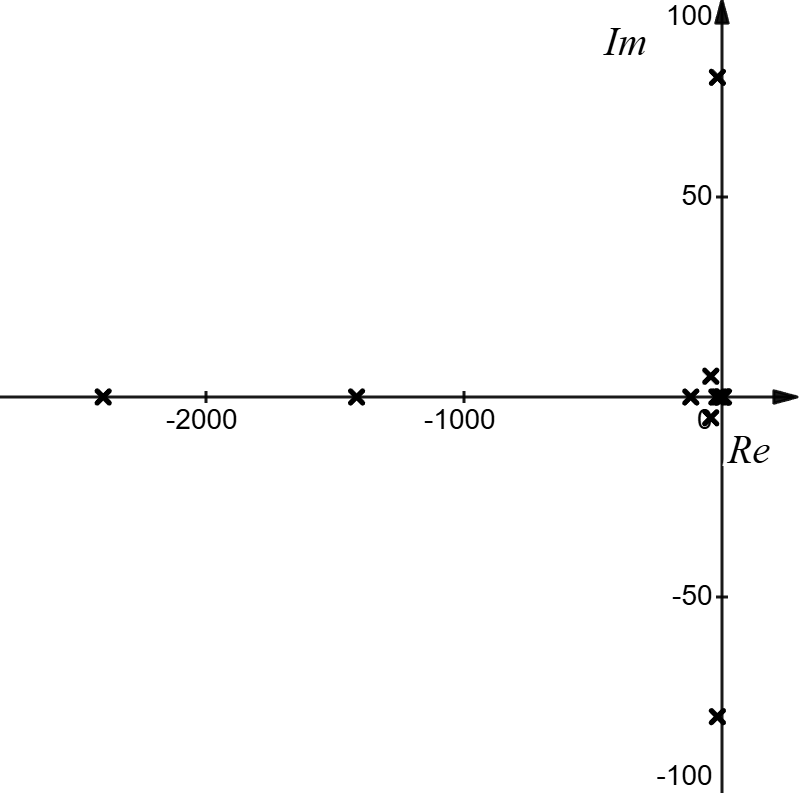
\includegraphics[width=.95\textwidth]{png/roots1.png}
	 		\caption{}
	 	\end{subfigure}
	 	\begin{subfigure}{.5\textwidth}
	 		\centering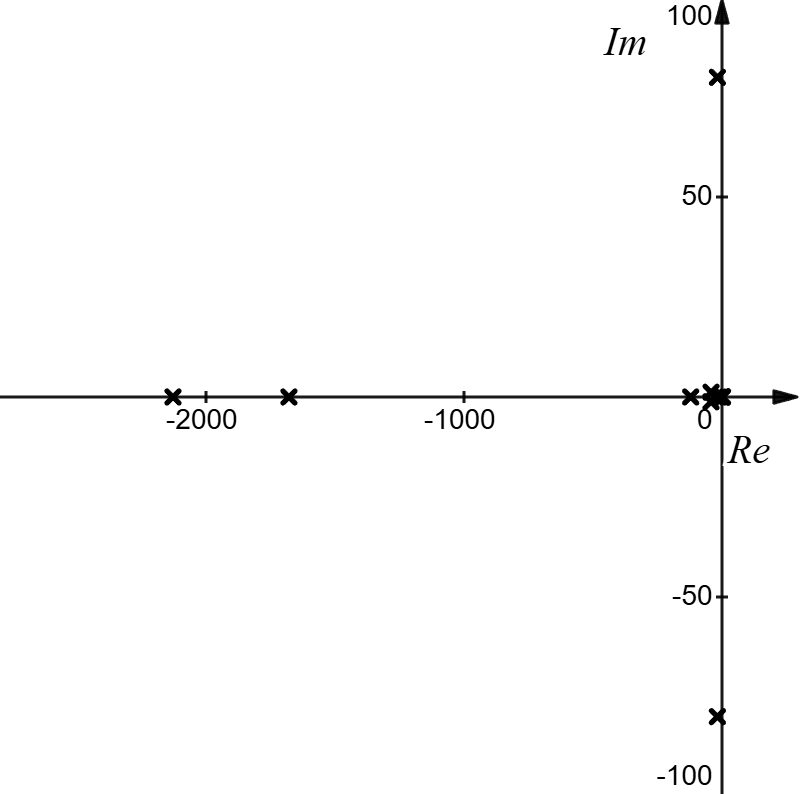
\includegraphics[width=.95\textwidth]{png/roots2.png}
	 		\caption{}
	 	\end{subfigure}
	 	\caption{Собственные значения матрицы Якоби: а) $t=T_i=0,3$ с; б) $t=T_j=1$ с}
	 	\label{roots} 
	\end{figure}
	
	Сами матрицы Якоби, по которым рассчитывались спектры:
	\begin{equation*}
		\scalemath{0.55}{
		J_\varphi(T_i) = \begin{bmatrix}
			-2071.132  &  1014.733  &  1014.733  &  -318.25855  &  0  &  0  &  0  &  0  &  0  &  0  &  0  &  -148.80159\\
			3.034  &  -6.193  &  3.34  &  0  &  0  &  0  &  0  &  0  &  0.378  &  0  &  0  &  0\\
			78.069  &  78.069  &  -159.344  &  0  &  0  &  0  &  0  &  0  &  0  &  0  &  0  &  0\\
			-671.58681  &  0  &  0  &  -1606.256  &  1479.609  &  0  &  0  &  0  &  0  &  0  &  0  &  -40.323067\\
			0  &  0  &  0  &  97.31  &  -105.64  &  0  &  0  &  0  &  0  &  0  &  0  &  0\\
			0  &  0  &  0  &  0  &  0  &  0  &  1  &  0  &  0  &  0  &  0  &  0\\
			0  &  0  &  0  &  0  &  0  &  0  &  0  &  1  &  0  &  0  &  0  &  0\\
			0  &  0  &  0  &  0  &  0  &  -33949.6  &  -6989.92  &  -45  &  0  &  0  &  0  &  -100000\\
			0  &  0  &  0  &  0  &  0  &  0  &  0  &  0  &  0  &  1  &  0  &  0\\
			0  &  0  &  0  &  0  &  0  &  0  &  0  &  0  &  0  &  0  &  1  &  0\\
			350321  &  -171734.38  &  -171734.38  &  271819.97  &  -250406.71  &  0  &  0  &  0  &  -55555.55  &  -4444.44  &  -116.66  &  0\\
			-1.069571  &  0.57577685  &  0.57577685  &  -0.62722537  &  0.22729882  &  0.303  &  0  &  0  &  0  &  0  &  0  &  0
		\end{bmatrix}}
	\end{equation*}
	
	\begin{equation*}
		\scalemath{0.53}{
		J_\varphi(T_j) = \begin{bmatrix}
			-2071.132  &  1014.733  &  1014.733  &  -15.802703  &  0  &  0  &  0  &  0  &  0  &  0  &  0  &  -10.195748\\
			3.034  &  -6.193  &  3.34  &  0  &  0  &  0  &  0  &  0  &  0.378  &  0  &  0  &  0\\
			78.069  &  78.069  &  -159.344  &  0  &  0  &  0  &  0  &  0  &  0  &  0  &  0  &  0\\
			-486.67827  &  0  &  0  &  -1606.256  &  1479.609  &  0  &  0  &  0  &  0  &  0  &  0  &  -4.1245303\\
			0  &  0  &  0  &  97.31  &  -105.64  &  0  &  0  &  0  &  0  &  0  &  0  &  0\\
			0  &  0  &  0  &  0  &  0  &  0  &  1  &  0  &  0  &  0  &  0  &  0\\
			0  &  0  &  0  &  0  &  0  &  0  &  0  &  1  &  0  &  0  &  0  &  0\\
			0  &  0  &  0  &  0  &  0  &  -33949.6  &  -6989.92  &  -45  &  0  &  0  &  0  &  -100000\\
			0  &  0  &  0  &  0  &  0  &  0  &  0  &  0  &  0  &  1  &  0  &  0\\
			0  &  0  &  0  &  0  &  0  &  0  &  0  &  0  &  0  &  0  &  1  &  0\\
			336210  &  -164816.88  &  -164816.88  &  260871.01  &  -240320.28  &  0  &  0  &  0  &  -55555.55  &  -4444.44  &  -116.66  &  0\\
			-0.072747756  &  0.039451699  &  0.039451699  &  -0.044119862  &  0.023249741  &  0.303  &  0  &  0  &  0  &  0  &  0  &  0
		\end{bmatrix}}
	\end{equation*}

	\section{Выводы}
	
	В этой работе было проведено моделирование нелинейной системы 12 порядка, заданной в переменных состояния. Исследуемая система оказалась устойчива по входному ступенчатому воздействию, а в процессе свободного движения система приходила в точку покоя, находящуюся в нуле.
	
	Была проведена проверка принадлежности системы к классу сингулярно-возмущённых в два момента времени $T_i=0,3$ с и $T_j = 1$ с, при условии, что в качестве начальных условий задан установившийся режим для ступенчатого входного воздействия.
	
	Система оказалась сингулярно-возмущённой в окрестности $x(T_i)$ и $x(T_j)$. В обоих случаях всего было два <<выделяющихся>> собственных значения, поэтому порядок системы может быть понижен на два.

\end{document}
